% \definecolor{azure}{rgb}{0.0, 0.5, 1.0}
% \definecolor{awesome}{rgb}{1.0, 0.13, 0.32}
% \definecolor{amber}{rgb}{1.0, 0.49, 0.0}
%\definecolor{darkpastelgreen}{rgb}{0.01, 0.75, 0.24}
\definecolor{mycolor1}{rgb}{0.85,0.325,0.098}
\definecolor{mycolor2}{rgb}{0.00000,0.44700,0.74100}
\definecolor{mycolor3}{rgb}{0.00000,0.49804,0.00000}

\definecolor{apricot}{rgb}{0.98, 0.81, 0.69}
\definecolor{copper}{rgb}{0.72, 0.45, 0.2}
\definecolor{babyblue}{rgb}{0.54, 0.81, 0.94}
\definecolor{gray}{rgb}{0.5, 0.5, 0.5}
\usetikzlibrary{decorations.pathreplacing}
\linespread{0.6}
\tikzstyle{startstop} = [rectangle, rounded corners, minimum width=1.5cm, minimum height=0.8cm,text centered, draw=black, fill=mycolor1!20, inner sep=-0.3ex]
\tikzstyle{startstop_blue} = [rectangle, rounded corners, minimum width=1.5cm, minimum height=0.8cm,text centered, draw=black, fill=mycolor2!20, inner sep=-0.3ex]
\tikzstyle{startstop_green} = [rectangle, rounded corners, minimum width=1.5cm, minimum height=0.8cm,text centered, draw=black, fill=mycolor3!20, inner sep=-0.3ex]

% \tikzstyle{io} = [trapezium, trapezium left angle=70, trapezium right angle=110, minimum width=3cm, minimum height=1cm, text centered, draw=black, fill=blue!30]
%\tikzstyle{process} = [rectangle, minimum width=3cm, minimum height=0.8cm, text centered, draw=black, fill=orange!30, inner sep=-0.3ex]
\tikzstyle{decision} = [diamond, aspect=2,  text centered, draw=black, fill=mycolor1!20, inner sep=-0.3ex]
\tikzstyle{arrow} = [thick,->,>=stealth]

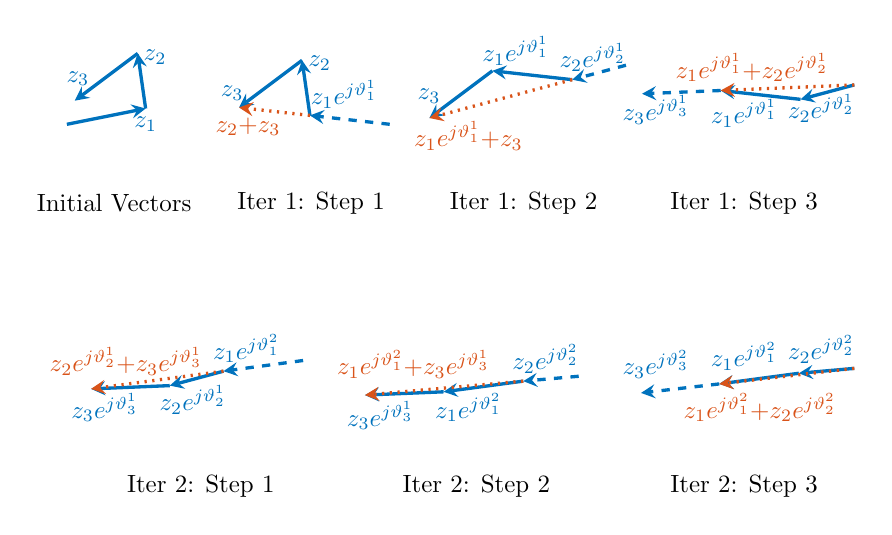
\begin{tikzpicture}[cross/.style={path picture={ 
  \draw[black]
(path picture bounding box.south east) -- (path picture bounding box.north west) (path picture bounding box.south west) -- (path picture bounding box.north east);
}}]



%\node (in1) [io, below of=start] {Input};

%\node (pro1) [process, below of=in1] {Process 1};


\pgfmathsetmacro{\xshift}{4.1}
\pgfmathsetmacro{\xshiftt}{7.1}
\pgfmathsetmacro{\yshiftt}{0.75}

\pgfmathsetmacro{\xshifttt}{10}
\pgfmathsetmacro{\yshifttt}{0.5}


\draw[arrow, color = mycolor2, line width = 1.2] (0,0) -- (1,0.2);
\draw[arrow, color = mycolor2, line width = 1.2] (1,0.2) -- (0.9,0.9);
\draw[arrow, color = mycolor2, line width = 1.2] (0.9,0.9) -- (0.1,0.3);
\node[mycolor2] at (1, 0) {\scalebox{0.9}{$z_{1}$}};
\node[mycolor2] at (1.12, 0.85) {\scalebox{0.9}{$z_{2}$}};
\node[mycolor2] at (0.14, 0.58) {\scalebox{0.9}{$z_{3}$}};


\draw[arrow, color = mycolor2, dashed, line width = 1.2] (\xshift+0,0) -- (\xshift-1.0136,0.1126);
\draw[arrow, color = mycolor2, line width = 1.2] (\xshift-1.0136,0.1126) -- (\xshift-1.1136,0.8126);
\draw[arrow, color = mycolor2, line width = 1.2] (\xshift-1.1136,0.8126) -- (\xshift-1.9136,0.2126);
\draw[arrow, color = mycolor1, dotted, line width = 1.2] (\xshift-1.0136,0.1126) -- (\xshift-1.9136,0.2126);
\node[mycolor2] at (\xshift-0.58, 0.38) {\scalebox{0.9}{$z_{1}e^{j\vartheta^{1}_{1}}$}};
\node[mycolor2] at (\xshift-0.89, 0.78) {\scalebox{0.9}{$z_{2}$}};
\node[mycolor2] at (\xshift-2, 0.4) {\scalebox{0.9}{$z_{3}$}};
\node[mycolor1] at (\xshift-1.8, -0.03) {\scalebox{0.9}{$z_{2}{+}z_{3}$}};



\draw[arrow, color = mycolor2, dashed, line width = 1.2] (\xshiftt+0,\yshiftt+0) -- (\xshiftt-0.6829,\yshiftt- 0.1835);
\draw[arrow, color = mycolor2, line width = 1.2] (\xshiftt-0.6829,\yshiftt- 0.1835) -- (\xshiftt-1.6964,\yshiftt- 0.0709);
\draw[arrow, color = mycolor2, line width = 1.2] (\xshiftt-1.6964,\yshiftt- 0.0709) -- (\xshiftt-2.4964,\yshiftt- 0.6709);
\draw[arrow, color = mycolor1, dotted, line width = 1.2] (\xshiftt-0.6829,\yshiftt- 0.1835) -- (\xshiftt-2.4964,\yshiftt- 0.6709);
\node[mycolor2] at (\xshiftt-1.4, \yshiftt+0.18) {\scalebox{0.9}{$z_{1}e^{j\vartheta^{1}_{1}}$}};
\node[mycolor2] at (\xshiftt-0.42, \yshiftt+0.10) {\scalebox{0.9}{$z_{2}e^{j\vartheta^{1}_{2}}$}};
\node[mycolor2] at (\xshiftt-2.5, \yshiftt-0.39) {\scalebox{0.9}{$z_{3}$}};
\node[mycolor1] at (\xshiftt-2, \yshiftt-0.9) {\scalebox{0.9}{$z_{1}e^{j\vartheta^{1}_{1}}{+}z_{3}$}};



\draw[arrow, color = mycolor2, line width = 1.2] (\xshifttt+0,\yshifttt+0) -- (\xshifttt-0.6829,\yshifttt- 0.1835);
\draw[arrow, color = mycolor2, line width = 1.2] (\xshifttt-0.6829,\yshifttt- 0.1835) -- (\xshifttt-1.6964,\yshifttt- 0.0709);
\draw[arrow, color = mycolor2, dashed, line width = 1.2] (\xshifttt-1.6964,\yshifttt- 0.0709) -- (\xshifttt-2.6956,\yshifttt- 0.1127);
\draw[arrow, color = mycolor1, dotted, line width = 1.2] (\xshifttt+0,\yshifttt+0) -- (\xshifttt-1.6964,\yshifttt- 0.0709);
\node[mycolor2] at (\xshifttt-1.4, \yshifttt-0.36) {\scalebox{0.9}{$z_{1}e^{j\vartheta^{1}_{1}}$}};
\node[mycolor2] at (\xshifttt-0.42, \yshifttt-0.30) {\scalebox{0.9}{$z_{2}e^{j\vartheta^{1}_{2}}$}};
\node[mycolor2] at (\xshifttt-2.52, \yshifttt-0.32) {\scalebox{0.9}{$z_{3}e^{j\vartheta^{1}_{3}}$}};
\node[mycolor1] at (\xshifttt-1.3, \yshifttt+0.22) {\scalebox{0.9}{$z_{1}e^{j\vartheta^{1}_{1}}{+}z_{2}e^{j\vartheta^{1}_{2}}$}};



%% Iteration 2

\pgfmathsetmacro{\xshiftttt}{3}
\pgfmathsetmacro{\yshiftttt}{-3}


\draw[arrow, color = mycolor2, dashed, line width = 1.2] (\xshiftttt+0,\yshiftttt+0) -- (\xshiftttt-1.0108,\yshiftttt - 0.1354);
\draw[arrow, color = mycolor2, line width = 1.2] (\xshiftttt-1.0108,\yshiftttt - 0.1354) -- (\xshiftttt-1.6937,\yshiftttt- 0.3189);
\draw[arrow, color = mycolor2, line width = 1.2] (\xshiftttt-1.6937,\yshiftttt- 0.3189) -- (\xshiftttt-2.6928,\yshiftttt- 0.3606);
\draw[arrow, color = mycolor1, dotted, line width = 1.2] (\xshiftttt-1.0108,\yshiftttt - 0.1354) -- (\xshiftttt-2.6928,\yshiftttt- 0.3606);
\node[mycolor2] at (\xshiftttt-0.72, \yshiftttt+0.15) {\scalebox{0.9}{$z_{1}e^{j\vartheta^{2}_{1}}$}};
\node[mycolor2] at (\xshiftttt-1.4, \yshiftttt-0.5) {\scalebox{0.9}{$z_{2}e^{j\vartheta^{1}_{2}}$}};
\node[mycolor2] at (\xshiftttt-2.52, \yshiftttt-0.6) {\scalebox{0.9}{$z_{3}e^{j\vartheta^{1}_{3}}$}};
\node[mycolor1] at (\xshiftttt-2.25, \yshiftttt-0.01) {\scalebox{0.9}{$z_{2}e^{j\vartheta^{1}_{2}}{+}z_{3}e^{j\vartheta^{1}_{3}}$}};



\pgfmathsetmacro{\xshifttttt}{6.5}
\pgfmathsetmacro{\yshifttttt}{-3.2}


\draw[arrow, color = mycolor2, dashed, line width = 1.2] (\xshifttttt+0,\yshifttttt+0) -- (\xshifttttt-0.7044,\yshifttttt - 0.0621);
\draw[arrow, color = mycolor2, line width = 1.2] (\xshifttttt-0.7044,\yshifttttt - 0.0621) -- (\xshifttttt-1.7152,\yshifttttt- 0.1975);
\draw[arrow, color = mycolor2, line width = 1.2] (\xshifttttt-1.7152,\yshifttttt- 0.1975) -- (\xshifttttt-2.7143,\yshifttttt- 0.2392);
\draw[arrow, color = mycolor1, dotted, line width = 1.2] (\xshifttttt-0.7044,\yshifttttt - 0.0621) -- (\xshifttttt-2.7143,\yshifttttt- 0.2392);
\node[mycolor2] at (\xshifttttt-1.4, \yshifttttt-0.4) {\scalebox{0.9}{$z_{1}e^{j\vartheta^{2}_{1}}$}};
\node[mycolor2] at (\xshifttttt-0.42, \yshifttttt+0.22) {\scalebox{0.9}{$z_{2}e^{j\vartheta^{2}_{2}}$}};
\node[mycolor2] at (\xshifttttt-2.52, \yshifttttt-0.5) {\scalebox{0.9}{$z_{3}e^{j\vartheta^{1}_{3}}$}};
\node[mycolor1] at (\xshifttttt-2.1, \yshifttttt+0.15) {\scalebox{0.9}{$z_{1}e^{j\vartheta^{2}_{1}}{+}z_{3}e^{j\vartheta^{1}_{3}}$}};


\pgfmathsetmacro{\xshiftttttt}{10}
\pgfmathsetmacro{\yshiftttttt}{-3.1}


\draw[arrow, color = mycolor2, line width = 1.2] (\xshiftttttt+0,\yshiftttttt+0) -- (\xshiftttttt-0.7044,\yshiftttttt - 0.0621);
\draw[arrow, color = mycolor2, line width = 1.2] (\xshiftttttt-0.7044,\yshiftttttt - 0.0621) -- (\xshiftttttt-1.7152,\yshiftttttt- 0.1975);
\draw[arrow, color = mycolor2, dashed, line width = 1.2] (\xshiftttttt-1.7152,\yshiftttttt- 0.1975) -- (\xshiftttttt - 2.7086,\yshiftttttt- 0.3118);
\draw[arrow, color = mycolor1, dotted, line width = 1.2] (\xshiftttttt+0,\yshiftttttt+0) -- (\xshiftttttt-1.7152,\yshiftttttt- 0.1975);
\node[mycolor2] at (\xshiftttttt-1.4, \yshiftttttt+0.15) {\scalebox{0.9}{$z_{1}e^{j\vartheta^{2}_{1}}$}};
\node[mycolor2] at (\xshiftttttt-0.42, \yshiftttttt+0.24) {\scalebox{0.9}{$z_{2}e^{j\vartheta^{2}_{2}}$}};
\node[mycolor2] at (\xshiftttttt-2.52, \yshiftttttt+0.05) {\scalebox{0.9}{$z_{3}e^{j\vartheta^{2}_{3}}$}};
\node[mycolor1] at (\xshiftttttt-1.2, \yshiftttttt-0.5) {\scalebox{0.9}{$z_{1}e^{j\vartheta^{2}_{1}}{+}z_{2}e^{j\vartheta^{2}_{2}}$}};



\node[black] at (0.6, -1) {\scalebox{0.9}{Initial Vectors}};
\node[black] at (3.1, -1) {\scalebox{0.9}{Iter 1: Step 1}};
\node[black] at (5.8, -1) {\scalebox{0.9}{Iter 1: Step 2}};
\node[black] at (8.6, -1) {\scalebox{0.9}{Iter 1: Step 3}};


\node[black] at (1.7, -4.6) {\scalebox{0.9}{Iter 2: Step 1}};
\node[black] at (5.2, -4.6) {\scalebox{0.9}{Iter 2: Step 2}};
\node[black] at (8.6, -4.6) {\scalebox{0.9}{Iter 2: Step 3}};

\end{tikzpicture}

